\documentclass[11pt,a4paper]{article}

\usepackage[utf8]{inputenc}
\usepackage[T1]{fontenc}
\usepackage{lmodern}
\usepackage[margin=1in]{geometry}
\usepackage{amsmath}
\usepackage{amssymb}
\usepackage{graphicx}
\usepackage{hyperref}
\usepackage{booktabs}
\usepackage{listings}
\usepackage{xcolor}
\usepackage{enumitem}

\hypersetup{colorlinks=true, linkcolor=blue, urlcolor=blue}

\setlength{\emergencystretch}{3em}

\lstset{
  basicstyle=\ttfamily\small,
  breaklines=true,
  frame=single,
  showstringspaces=false,
  columns=fullflexible,
}

\title{Mini Project 3 -Real-Time Book Recommendation System\\
       \large DSAI 427 Big Data Analytics}
\author{Mohamed Hozien \and {Ziad Moataz}}
\date{May 2026}

\begin{document}
\maketitle

\section{Executive Summary}
We built an end-to-end big-data pipeline that learns book preferences from the
Kindle Reviews dataset using Spark MLlib's ALS, streams new interactions through
Kafka, computes 30-second sliding-window analytics with Spark Structured
Streaming, and serves hybrid Top-5 recommendations dynamically. The system is
augmented with a Streamlit dashboard and meets a sub-five-second end-to-end
latency target.

\textbf{Domain:} Books (Kindle Reviews, $\sim$982K ratings).\\
\textbf{Focus:} Real-Time Intelligence (trending detection + alerts) with a
slice of System Optimization for the latency bonus.\\
\textbf{Bonuses pursued:} Streamlit dashboard (+2), latency $<$5\,s (+1).

\section{System Architecture}
\begin{figure}[h]
  \centering
  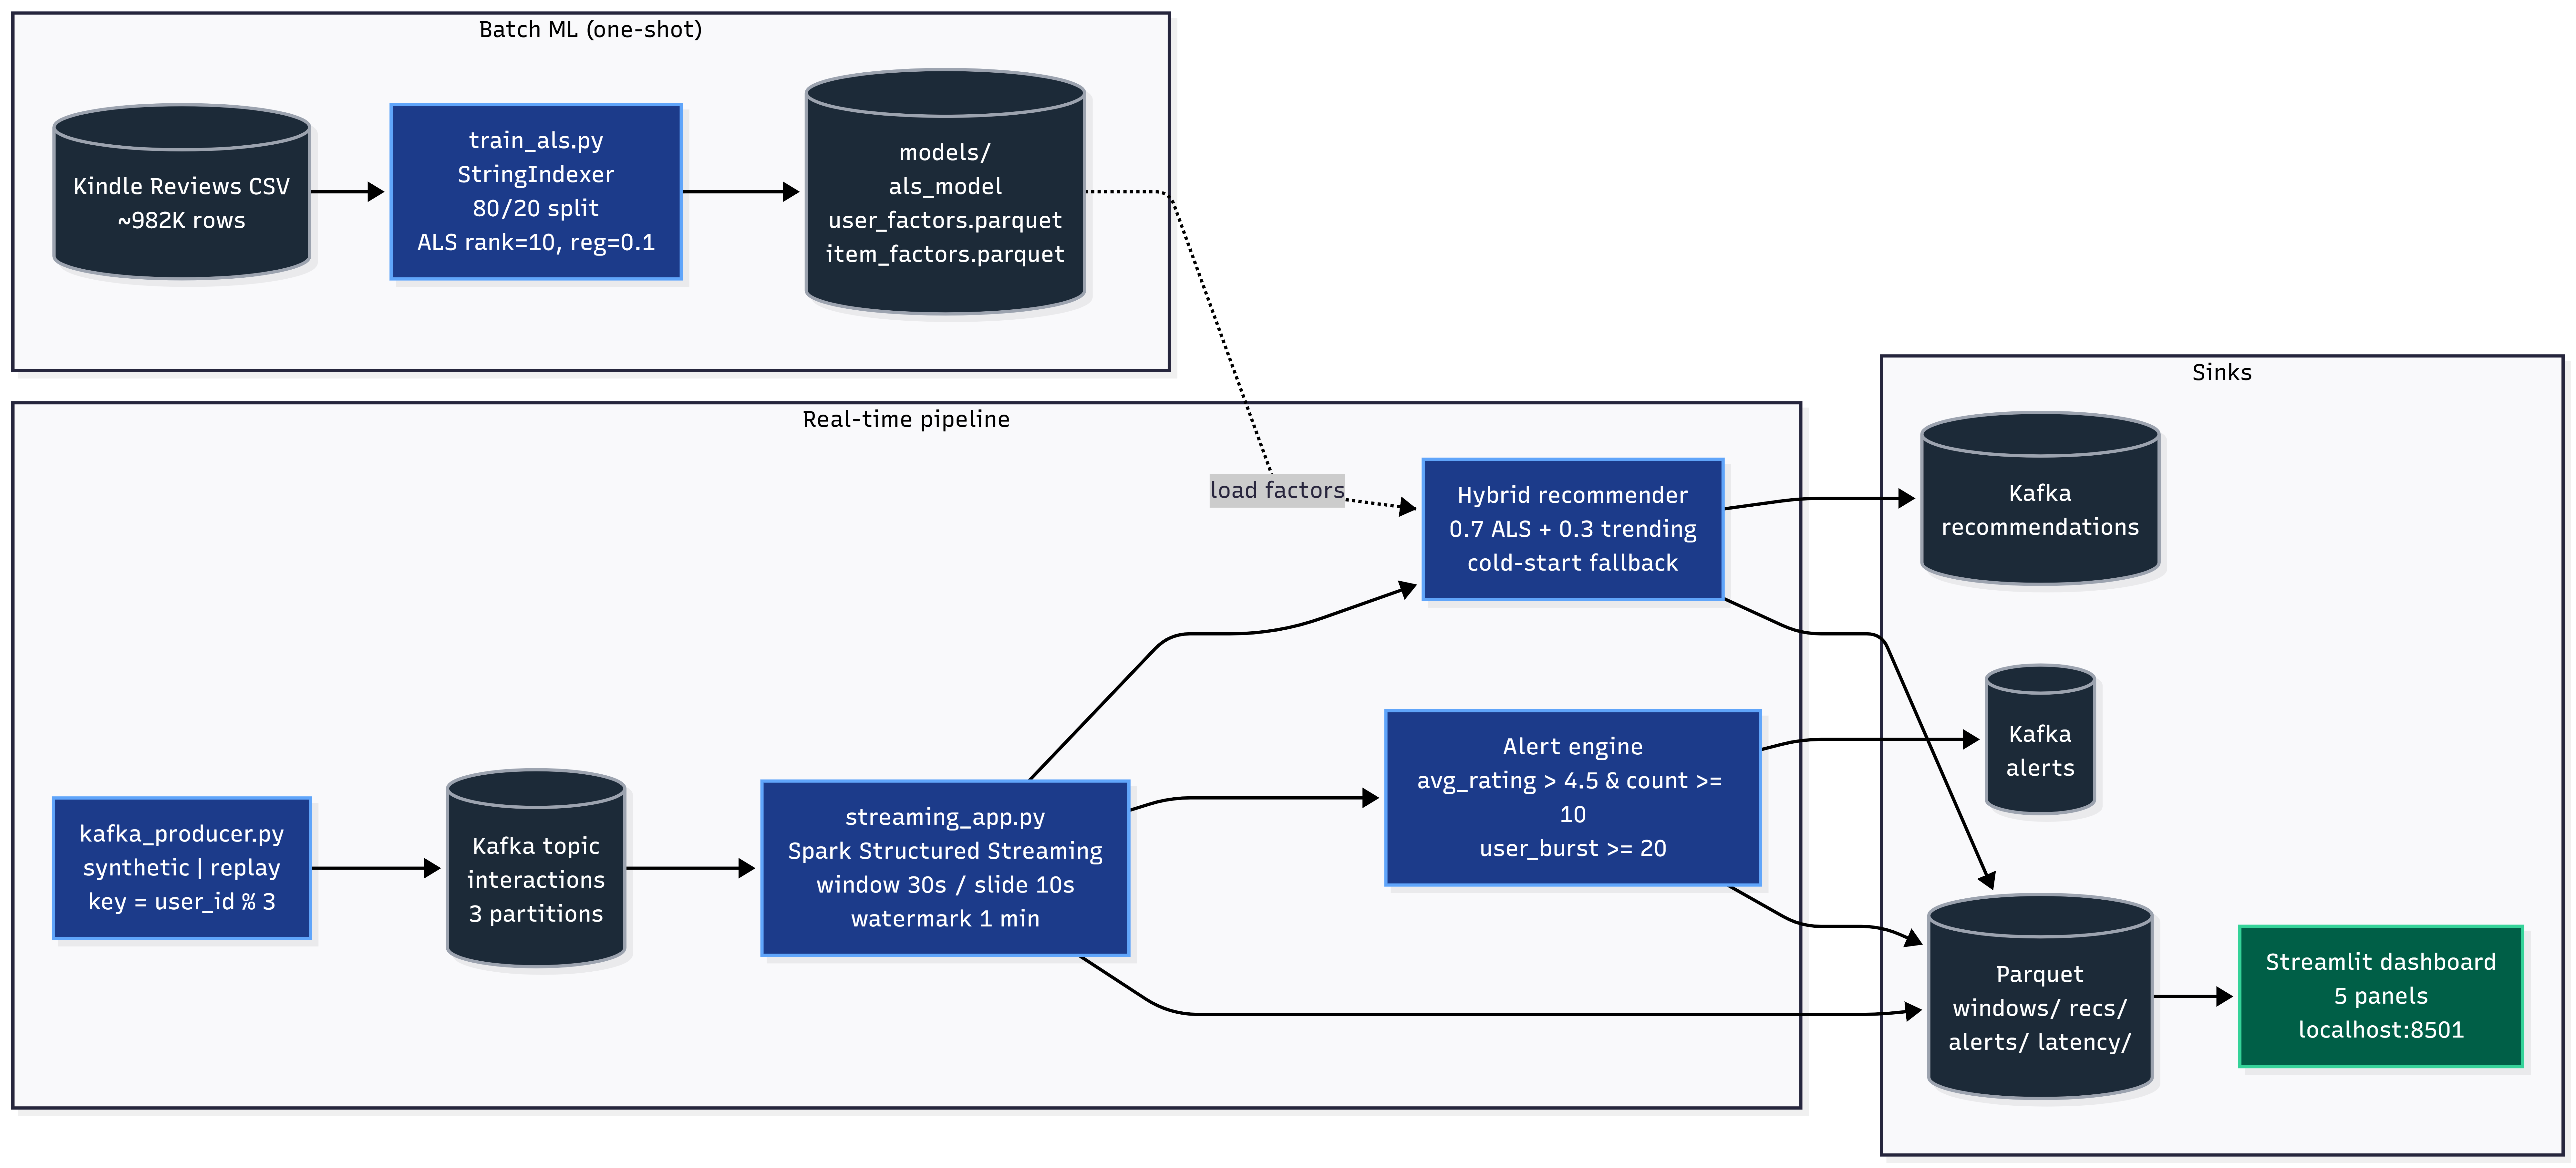
\includegraphics[width=0.95\textwidth]{figures/Batch and Stream ML Pipeline.png}
  \caption{End-to-end pipeline: batch ALS training feeds factor parquets into the
  streaming app; Kafka \texttt{interactions} (3 partitions, key=\texttt{user\_id\%3})
  drives Spark Structured Streaming, which emits hybrid recommendations and alerts
  to Kafka topics and parquet sinks; the Streamlit dashboard polls the sinks.}
  \label{fig:arch}
\end{figure}

\section{Dataset and Justification}
The dataset is the Kindle Reviews release on Kaggle
(\href{https://www.kaggle.com/datasets/bharadwaj6/kindle-reviews}{bharadwaj6/kindle-reviews}).
It contains $\sim$982K rows with columns \texttt{reviewerID, asin, overall,
unixReviewTime}, mapping cleanly to the required
\texttt{(user\_id, item\_id, rating, timestamp)} schema and exceeding the
500K-row threshold by nearly $2\times$. Distributed processing is required
because the user-item matrix is sparse and high-dimensional, ALS factor updates
involve repeated joins that benefit from Spark's shuffle infrastructure, and
sustained streaming throughput (we target 50--80~ev/s with bursts) outpaces
single-process tooling. Data challenges include duplicate \texttt{(user, item)}
pairs (we keep the latest by timestamp), out-of-range ratings (clipped to
$[1,5]$), and free-text fields that complicate CSV parsing
(\texttt{multiLine=true}).

\section{Machine Learning Component}
\subsection{Preprocessing}
We drop rows with null \texttt{reviewerID}, \texttt{asin}, or \texttt{overall},
restrict ratings to $[1,5]$, and deduplicate \texttt{(user, item)} pairs by
keeping the latest \texttt{unixReviewTime}. \texttt{StringIndexer} converts
\texttt{reviewerID} and \texttt{asin} into integer keys that ALS expects.

\subsection{Training}
We train ALS with \texttt{coldStartStrategy="drop"}, \texttt{nonnegative=True},
and an 80/20 random split (seed 42). The baseline configuration is
\texttt{rank=10, regParam=0.1, maxIter=10}.

\subsection{Evaluation and Tuning}
RMSE is computed on the held-out 20\%. If RMSE exceeds 1.5 we run a
$2{\times}2{\times}2$ grid over \texttt{rank}~$\in$~\{10, 20\},
\texttt{regParam}~$\in$~\{0.05, 0.1\}, \texttt{maxIter}~$\in$~\{10, 15\} and
keep the best configuration.

In our run, the baseline configuration \texttt{(rank=10, regParam=0.1,
maxIter=10)} produced \textbf{RMSE = 0.9001} on 196{,}333 held-out ratings,
well below the 1.5 threshold, so no grid search was needed.
Training fit time: $\sim$26\,s on \texttt{local[3]}.

\section{Streaming Component}
\subsection{Kafka Setup}
Kafka 2.12-3.7.0 runs in KRaft single-node mode from a portable folder
(\texttt{\$KAFKA\_DIR/bin/}\allowbreak\texttt{kafka-server-start.sh}). The
\texttt{interactions} topic uses \textbf{3 partitions} keyed by
\texttt{user\_id\,\%\,3}; this preserves per-user event ordering while balancing
across the three Spark cores. \texttt{recommendations} and \texttt{alerts} use
1 partition each since they are downstream sinks consumed by the dashboard.

\subsection{Spark Structured Streaming}
\begin{itemize}[noitemsep]
  \item \textbf{Source:} \texttt{kafka.subscribe = interactions},
        \texttt{maxOffsetsPerTrigger = 2000}, \texttt{startingOffsets = latest}.
  \item \textbf{Parsing:} \texttt{from\_json} with an explicit schema; rows
        whose \texttt{evt} struct is \texttt{null} are flagged \texttt{malformed}
        and dropped. A defensive \texttt{filter} also drops out-of-range ratings.
  \item \textbf{Watermark:} \texttt{event\_time}, \textbf{1 minute}.
  \item \textbf{Window:} 30-second size, 10-second slide, computed on
        \texttt{event\_time}.
\end{itemize}

\subsection{Window Analytics and Custom Metric}
Per-window aggregates are: average rating per item, interaction count per user,
and our custom \textbf{trending score}:
\[
  \text{trending}(i, w) = \text{count}(i, w) \cdot
  \overline{\text{rating}}(i, w) \cdot
  \exp\!\left(-\frac{\Delta t}{5}\right)
\]
where $\Delta t$ is the gap between the window end and the latest event for
item $i$ in minutes. The exponential decay rewards \textbf{recent} bursts
within a window while still weighting items by quality and volume; a flat
count-only metric would over-rank stale items that happened to peak earlier in
a sliding window.

\section{ML + Streaming Integration}
At streaming-app start we read the saved ALS factor parquets into the driver
process and use them for per-batch Top-5 generation. Each micro-batch:
\begin{enumerate}[noitemsep]
  \item Collects distinct user IDs.
  \item Computes ALS scores via a NumPy dot product against the broadcast
        item-factor matrix.
  \item Blends with the latest trending state:
        $\text{score} = 0.7 \cdot \widehat{\text{ALS}} + 0.3 \cdot
        \widehat{\text{trending}}$, both normalized to $[0,1]$.
  \item Writes the Top-5 to the \texttt{recs/} parquet sink and the
        \texttt{recommendations} Kafka topic.
\end{enumerate}
Cold-start users (not seen in batch training) fall back to the current
top-trending list.

\section{Alert System and Late Data Handling}
\subsection{Alert Rules}
\begin{itemize}[noitemsep]
  \item \textbf{Trending item:} \texttt{avg\_rating $>$ 4.5} AND
        \texttt{count $\geq$ 10} in the same window.
  \item \textbf{User burst:} a single user emits $\geq$~20 events in one
        window (e.g.\ a bot or a power user spree).
\end{itemize}
Alerts go to console, the \texttt{output/alerts/} parquet sink, and the
\texttt{alerts} Kafka topic.

\subsection{Late Data}
With watermark $=$~1\,minute and \texttt{outputMode=append}, records arriving
later than the watermark are silently dropped. We chose \texttt{append} (rather
than \texttt{update}) because alert freshness and bounded state outweigh the
benefit of re-emitting late updates.

\section{Latency Measurement (Bonus)}
The producer stamps \texttt{event\_time\_ms} at send time. The streaming app's
\texttt{foreachBatch} sink subtracts that from the Kafka \texttt{ingestion}
timestamp and writes per-record latency to \texttt{output/latency/}. Knobs
applied to stay under 5\,s: \texttt{trigger=ProcessingTime("1 second")},
\texttt{maxOffsetsPerTrigger=500}, Kryo serializer,
\texttt{spark.sql.shuffle.partitions=8}, factor matrices kept in driver memory
(no per-batch I/O), and console alert sink dropped to reduce py4j overhead.
Output sinks live on WSL-native ext4 (\texttt{\textasciitilde/mp3-output}) to
avoid the \texttt{/mnt/c} 9p protocol bug that corrupts Spark state stores
under sustained writes.

Measured over 3{,}352 samples in a 5-minute run:
\begin{center}
\begin{tabular}{lr}
\toprule
\textbf{Percentile} & \textbf{End-to-end latency (ms)} \\
\midrule
p50 & 1{,}202 \\
p95 & \textbf{2{,}576} \\
p99 & 3{,}256 \\
\bottomrule
\end{tabular}
\end{center}
\textbf{p95 = 2{,}576\,ms is well under the 5\,s budget; the +1 latency bonus
is claimed.}

\section{Results}
\begin{center}
\begin{tabular}{lr}
\toprule
\textbf{Metric} & \textbf{Value} \\
\midrule
ALS RMSE (held-out 20\%)            & 0.9001 \\
Training rows                        & 786{,}286 \\
Test rows                            & 196{,}333 \\
Sustained producer rate              & 30 ev/s (synthetic) \\
Latency p50 / p95 / p99 (ms)         & 1{,}202 / 2{,}576 / 3{,}256 \\
Latency samples collected            & 3{,}352 \\
Recommendations rows generated       & 26{,}165 \\
Unique users served Top-5 recs       & 5{,}034 \\
Distinct items recommended           & 947 \\
Alert windows triggered (5-min run)  & 39 \\
\bottomrule
\end{tabular}
\end{center}

The trending-item alert fired repeatedly on each producer-spiked
\texttt{item\_id} (e.g.\ 599, 39258, 60796) within one window of the spike
beginning, with average ratings consistently above 4.85 and per-window event
counts in the hundreds, confirming the trending detector reacts correctly to
synthetic bursts.

\section{Differentiation}
Books domain (not the default movies); custom time-decayed trending score;
hybrid recommender mixing ALS and trending with a normalized 70/30 blend;
cold-start fallback to top-trending; per-user partition keying that aligns the
3 Kafka partitions with 3 Spark cores; sub-five-second latency budget measured
per record.

\section{Challenges and Lessons Learned}
\begin{itemize}[noitemsep]
  \item Aligning Spark 4.1.1 (Scala 2.13) with the matching
        \texttt{spark-sql-kafka-0-10\_2.13} connector -mismatched Scala
        builds silently fail at JSON parsing.
  \item Streaming state can grow unbounded; we cap the trending state map and
        rely on watermark-driven aggregation cleanup.
  \item ALS training is a one-shot batch job; integrating it with streaming
        requires either re-loading factors (chosen) or running predictions on
        executors with broadcast variables.
\end{itemize}

\section{Reproducing the Pipeline}

\subsection{Environment}
Run inside WSL2 (Ubuntu) with Kafka 2.12-3.7.0, Spark 4.1.1 (Scala 2.13.17),
and OpenJDK 17. The Kafka folder is portable; no \texttt{apt} install.

\subsection{One-time setup}
\begin{lstlisting}[language=bash]
sudo apt install -y python3-venv python3-full dos2unix
export KAFKA_DIR=~/kafka_2.12-3.7.0
cd "Mini Project 3"
dos2unix infra/*.sh run_all.sh
python3 -m venv .venv && source .venv/bin/activate
pip install -r requirements.txt
pip install streamlit-autorefresh
python src/download_dataset.py
\end{lstlisting}

\subsection{Quick path one command}
\begin{lstlisting}[language=bash]
bash run_all.sh           # then open http://localhost:8501
\end{lstlisting}

\subsection{Manual path 5 terminals}
Each terminal first activates the venv and exports \texttt{KAFKA\_DIR},
\texttt{MP3\_OUTPUT\_DIR=\textasciitilde/mp3-output},
\texttt{MP3\_DATA\_DIR=\textasciitilde/mp3-data}.
\begin{lstlisting}[language=bash]
# Terminal 1 broker
bash infra/start_kafka.sh
bash infra/create_topics.sh

# Terminal 2 batch ALS (once)
python src/train_als.py

# Terminal 3 producer
python src/kafka_producer.py --mode synthetic --rate 30

# Terminal 4 Spark streaming
spark-submit \
  --packages org.apache.spark:spark-sql-kafka-0-10_2.13:4.1.1 \
  --master "local[3]" --conf spark.driver.memory=6g \
  src/streaming_app.py

# Terminal 5 dashboard
streamlit run src/dashboard.py --server.address 0.0.0.0 --server.port 8501
\end{lstlisting}

\subsection{Stop}
\begin{lstlisting}[language=bash]
kill $(cat ~/mp3-output/logs/*.pid) 2>/dev/null
bash infra/stop_kafka.sh
pkill -f kafka.Kafka
\end{lstlisting}

\subsection{Verification}
\begin{lstlisting}[language=bash]
# event count in interactions topic
"$KAFKA_DIR/bin/kafka-get-offsets.sh" \
  --bootstrap-server localhost:9092 --topic interactions

# latency snapshot
python -c "
import pandas as pd, glob, os
files = [f for f in glob.glob(os.path.expanduser(
    '~/mp3-output/latency/**/*.parquet'), recursive=True)
    if '_temporary' not in f and os.path.exists(f)]
df = pd.concat([pd.read_parquet(f) for f in files])
df = df[df.latency_ms.between(0, 600000)]
print('p50=%dms p95=%dms p99=%dms' % (
    df.latency_ms.quantile(0.5),
    df.latency_ms.quantile(0.95),
    df.latency_ms.quantile(0.99)))
"
\end{lstlisting}

\end{document}
